\section{Results}
\subsection{SAR-to-Optical Translation}
We validate the trained model on both qualitative and quantitative metrics to assess its capability for direct SAR-to-optical image translation. Unlike most prior work that generates only 3–4 optical bands, the trained Pix2Pix model produces all 13 Sentinel-2 spectral bands.

Figure~\ref{fig:qualitative_results_translation} presents some representative examples demonstrating the model's performance on diverse geographic and terrain conditions. In row (a), the model achieves strong color fidelity and accurately reconstructs spectral characteristics of vegetation and water bodies. Row (b) shows an urban scene where the model successfully delineates the city layout and captures the river traversing the area, preserving fine structural details. Row (c) demonstrates the model's ability to capture topographic features and surface relief variation from SAR backscatter intensity. Finally, row (d) depicts a coastal scene, where the model accurately reconstructs the land--water boundary and shoreline geometry while producing a plausible optical appearance. Across all examples, the generated optical images exhibit minimal artifacts and maintain structural consistency with ground truth.

\begin{figure}[H]
    \centering
    \setlength{\tabcolsep}{2pt} % horizontal padding between columns (same as ablation)
    \renewcommand{\arraystretch}{1.0} % vertical padding (same as ablation)

    \begin{tabular}{c *{3}{c}}
        % ------------------- Row 1 -------------------
         & (i) & (ii) & (iii) \\
        \textbf{(a)} &
        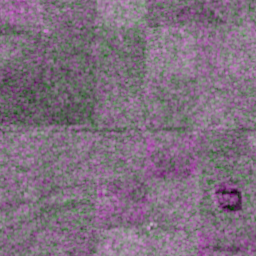
\includegraphics[width=0.2\textwidth, height=0.2\textheight, keepaspectratio]{../latex_source_code/img/qualitative-20-full/sample_1/sar.png} &
        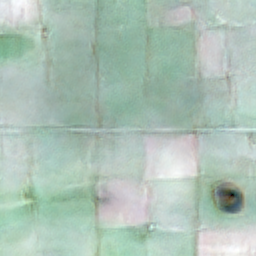
\includegraphics[width=0.2\textwidth, height=0.2\textheight, keepaspectratio]{../latex_source_code/img/qualitative-20-full/sample_1/gen_full.png} &
        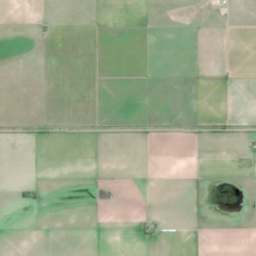
\includegraphics[width=0.2\textwidth, height=0.2\textheight, keepaspectratio]{../latex_source_code/img/qualitative-20-full/sample_1/gt.png} \\
        % ------------------- Row 2 -------------------
        \textbf{(b)} &
        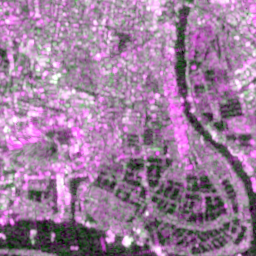
\includegraphics[width=0.2\textwidth, height=0.2\textheight, keepaspectratio]{../latex_source_code/img/qualitative-20-full/sample_2/sar.png} &
        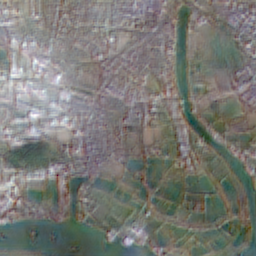
\includegraphics[width=0.2\textwidth, height=0.2\textheight, keepaspectratio]{../latex_source_code/img/qualitative-20-full/sample_2/gen_full.png} &
        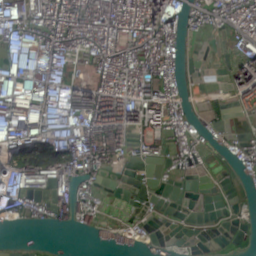
\includegraphics[width=0.2\textwidth, height=0.2\textheight, keepaspectratio]{../latex_source_code/img/qualitative-20-full/sample_2/gt.png} \\
        \textbf{(c)} &
        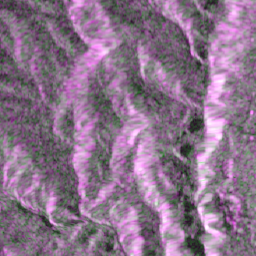
\includegraphics[width=0.2\textwidth, height=0.2\textheight, keepaspectratio]{../latex_source_code/img/qualitative-20-full/sample_3/sar.png} &
        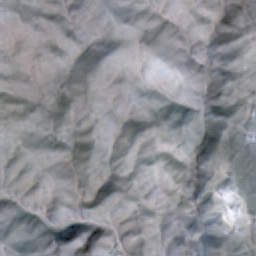
\includegraphics[width=0.2\textwidth, height=0.2\textheight, keepaspectratio]{../latex_source_code/img/qualitative-20-full/sample_3/gen_full.png} &
        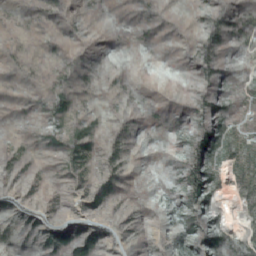
\includegraphics[width=0.2\textwidth, height=0.2\textheight, keepaspectratio]{../latex_source_code/img/qualitative-20-full/sample_3/gt.png} \\
        % ------------------- Row 4 -------------------
        \textbf{(d)} &
        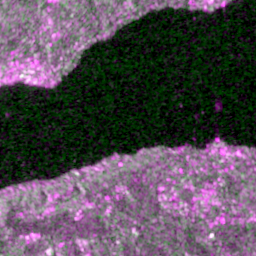
\includegraphics[width=0.2\textwidth, height=0.2\textheight, keepaspectratio]{../latex_source_code/img/qualitative-20-full/sample_4/sar.png} &
        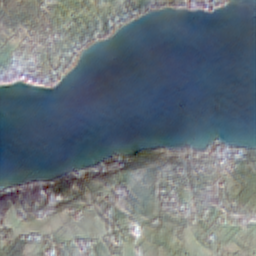
\includegraphics[width=0.2\textwidth, height=0.2\textheight, keepaspectratio]{../latex_source_code/img/qualitative-20-full/sample_4/gen_full.png} &
        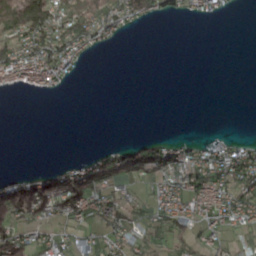
\includegraphics[width=0.2\textwidth, height=0.2\textheight, keepaspectratio]{../latex_source_code/img/qualitative-20-full/sample_4/gt.png} \\
    \end{tabular}

    \caption[Qualitative results on SAR-to-Optical Translation]{%
    Qualitative results on SAR-to-Optical Translation.
    Columns: \textbf{(i)}~SAR input (pseudo-RGB; R: VV, G: VH, B: VV/VH),
    \textbf{(ii)}~generated optical image, and
    \textbf{(iii)}~ground-truth Sentinel-2 image. For visualization purposes, all optical images are depicted in RGB (B4, B3, B2) batch.}
    \label{fig:qualitative_results_translation}
\end{figure}

To quantitatively assess the translation quality, we evaluate the model using standard image fidelity and spectral metrics (Table~\ref{tab:quantitative_result_translation}). The model achieves SSIM of 0.888 and PSNR of 32.63 dB across all 13 spectral bands, with excellent spectral angle mapper (SAM) of 4.41°, indicating strong preservation of spectral characteristics. These metrics are within the range reported for recent SAR-to-optical translation methods. Detailed quantitative comparison with state-of-the-art cloud removal methods is provided in Section~\ref{sec:cloud_removal}. 
% \textcolor{red}{TODO: add references}


\begin{table}[!htbp]
    \centering
    \caption{Quantitative results on SAR-to-Optical Translation.}
    \begin{tabular}{lccccc}
        \toprule
        \textbf{SSIM} & \textbf{PSNR (dB)} & \textbf{LPIPS} & \textbf{SAM (°)} & \textbf{MAE} & \textbf{RMSE} \\
        \midrule
        0.888           & 32.63                & 0.173              & 4.41                 & 140.72           & 233.69            \\
        \bottomrule
    \end{tabular}
    \label{tab:quantitative_result_translation}
\end{table}


These results demonstrate that the model effectively reconstructs full-spectrum optical imagery from SAR inputs with high fidelity across structural, spectral, and radiometric dimensions.

% \subsection{Across-Band Translation}
\subsection{Results Across Individual Optical Bands}
Another objective of this work was to assess the model’s ability to reliably reconstruct each optical band individually and to evaluate the uniformity of its accuracy across the spectrum. For this purpose, the trained model was evaluated separately for all 13 Sentinel-2 bands. The results are summarized in Table~\ref{tab:per_band_validation}.

When comparing reconstruction quality across bands, we focus on the Structural Similarity Index (SSIM). Unlike MAE or RMSE, which depend on the absolute magnitude and dynamic range of reflectance values (varying significantly between spectral bands), SSIM measures structural similarity based on local intensity patterns. While not entirely invariant to scale, SSIM provides a more robust and interpretable basis for cross-band comparison in this context.


\begin{table}[!htbp]
\centering
\caption{Per-band quantitative validation results. Each Sentinel-2 band’s central wavelength, spectral designation, and native spatial resolution are listed for reference. Best results are highlighted in \textcolor{green!50!black}{green} and worst in \textcolor{red!70!black}{red}. Arrows ($\uparrow$ / $\downarrow$) indicate whether higher or lower values denote better performance, respectively.}
\resizebox{0.9\textwidth}{!}{%
\begin{tabular}{lcccc}
\toprule
\textbf{Band} & \textbf{PSNR (dB) $\uparrow$} & \textbf{SSIM $\uparrow$} & \textbf{Central Wavelength [nm]} & \textbf{Spectral / Resolution [m]} \\
\midrule
B1   &  36.53  &  \cellcolor{green!15}\textbf{0.9758} & 443  & Aerosols / 60 \\
B2   &  \cellcolor{green!15}\textbf{37.49}  &  0.9506 & 490  & Blue / 10 \\
B3   &  35.67  &  0.9199 & 560  & Green / 10 \\
B4   &  32.84  &  0.8639 & 665  & Red / 10 \\
B5   &  33.68  &  0.9007 & 705  & Red Edge / 20 \\
B6   &  31.62  &  0.8536 & 740  & Red Edge / 20 \\
B7   &  30.37  &  0.8253 & 783  & Red Edge / 20 \\
B8   &  \cellcolor{red!15}\textit{29.62}  &  \cellcolor{red!15}\textit{0.7738} & 842  & NIR / 10 \\
B8A  &  29.62  &  0.8071 & 865  & Red Edge / 20 \\
B9   &  33.99  &  0.9388 & 945  & Water Vapour / 60 \\
B10  &  32.12  &  0.9386 & 1375 & Cirrus / 60 \\
B11  &  29.92  &  0.8309 & 1610 & SWIR / 20 \\
B12  &  31.48  &  0.8586 & 2190 & SWIR / 20 \\
\bottomrule
\end{tabular}% 
}
\label{tab:per_band_validation}
\end{table}
Notably, Band~8 (NIR), despite its native spatial resolution of 10~m, exhibits the lowest reconstruction performance among all spectral bands, including those with coarser resolutions, as illustrated in Figure~\ref{fig:ssim_per_band}. This indicates a weaker correlation between SAR backscatter and NIR reflectance compared to other spectral regions, likely due to their differing sensitivities to surface structure and vegetation properties. This limitation may also stem from the use of winter-only training samples, where vegetation-related information captured by the NIR band is comparatively scarce. 

In contrast, the 60~m atmospheric correction bands—B1 (Aerosols), B9 (Water Vapour), and B10 (Cirrus)—are reconstructed with high structural similarity. B1 achieves the highest SSIM overall (0.9758). This high performance likely stems from the lower spatial complexity and smoother textural characteristics of these bands compared to land-cover bands. The model can more easily recover these spatially homogeneous signals, even after they are upsampled to 10~m.


\begin{figure}[!htbp]
\centering
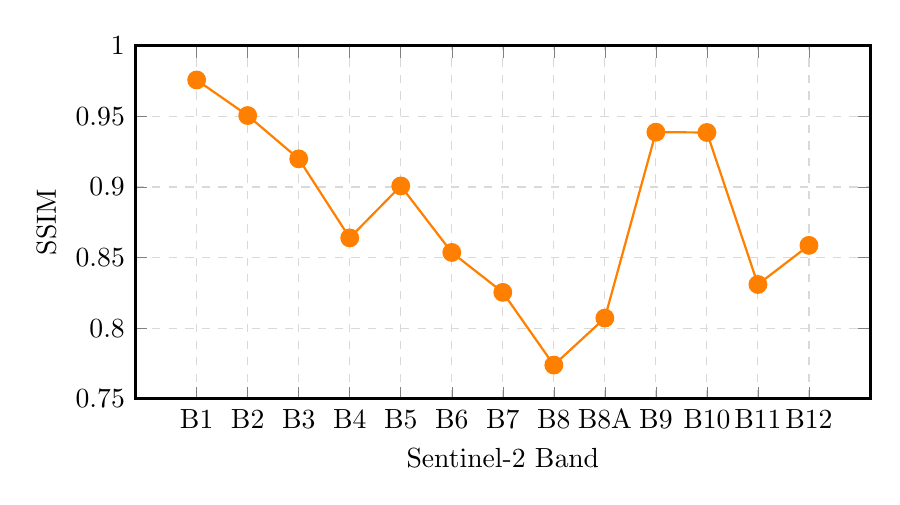
\begin{tikzpicture}
\begin{axis}[
    width=0.9\textwidth,
    height=0.5\textwidth,
    xlabel={Sentinel-2 Band},
    ylabel={SSIM},
    ymin=0.75, ymax=1.0,
    ytick distance=0.05,
    xtick=data,
    xticklabels={B1,B2,B3,B4,B5,B6,B7,B8,B8A,B9,B10,B11,B12},
    grid=major,
    grid style={dashed,gray!30},
    every axis plot/.append style={thick, mark=*},
    mark size=3pt,
    line width=1pt,
]

\addplot[
    color=orange,
    mark=*,
    mark options={fill=orange},
]
coordinates {
    (1,0.9758)
    (2,0.9506)
    (3,0.9199)
    (4,0.8639)
    (5,0.9007)
    (6,0.8536)
    (7,0.8253)
    (8,0.7738)
    (9,0.8071)
    (10,0.9388)
    (11,0.9386)
    (12,0.8309)
    (13,0.8586)
};

\end{axis}
\end{tikzpicture}
\caption[Per-band SSIM for the Pix2Pix model]{Per-band SSIM for the Pix2Pix model trained on the full winter subset.}
\label{fig:ssim_per_band}
\end{figure}

These findings, however, contrast with those reported in~\cite{CR_SEN2_dRNN}, where the authors observed that 10~m and 20~m bands achieved the highest reconstruction quality, while 60~m bands performed worst. However, their study employed an optical-SAR fusion approach on the full SEN12-MS-CR dataset. In their case, the presence of input optical channels likely allowed the model to exploit the high spatial detail of the 10~m bands directly. In our SAR-only translation setting, the model must synthesize optical textures purely from SAR structure; thus, it performs best on bands with lower spatial complexity (atmospheric bands) and struggles where SAR-optical physical correlation is weak.

To visually complement this quantitative assessment, representative grayscale examples for each Sentinel-2 band are provided in Appendix~\ref{appendix:bandwise_results}.

\subsection{Cloud Removal}
\label{sec:cloud_removal}
To evaluate the practical utility of the learned SAR-to-optical translation, we assess the model on the cloud removal task using the SEN12-MS-CR benchmark (Section~\ref{sec:datasets}). This dataset provides co-registered triplets: Sentinel-1 SAR, cloud-contaminated Sentinel-2 optical observations, and ground-truth cloud-free Sentinel-2 references. Since the SAR modality is unaffected by atmospheric conditions, mapping SAR to optical effectively bypasses cloud occlusion.

For quantitative evaluation, we employ a subset of 2{,}000 samples from the winter portion of SEN12-MS-CR. To ensure consistency with the training phase, this evaluation data undergoes the identical preprocessing and clipping steps described in Section~\ref{subsec:preprocessing}. Table~\ref{tab:quantitative_result_cr} presents the quantitative performance. Despite not being explicitly trained for cloud removal or on the SEN12-MS-CR dataset specifically, the proposed approach achieves strong results. The Spectral Angle Mapper (SAM) score of 3.86° indicates high spectral fidelity in the reconstructed observations, while the best-in-class PSNR (33.65 dB) and LPIPS (0.152) reflect superior reconstruction quality and perceptual similarity.

\begin{table}[!htbp]
    \centering
    \caption[Quantitative results on cloud removal against SOTA models]{Quantitative evaluation on SEN12-MS-CR for cloud removal.}
    \begin{tabular}{lcccc}
        \toprule
        \textbf{Model}                & \textbf{SSIM $\uparrow$} & \textbf{PSNR (dB) $\uparrow$} & \textbf{LPIPS $\downarrow$} & \textbf{SAM (°) $\downarrow$} \\
        \midrule
        DSen2-CR~\cite{CR_SEN2_dRNN}  & 0.878                    & --                            & --                          & 8.07                          \\
        FAT~\cite{c_guided_fus_s2ot}  & 0.880                    & 31.85                         & --                          & 4.19                          \\
        DiffCR~\cite{DiffCR}          & \textbf{0.902}           & 31.77                         & --                          & 5.82                          \\
        Pix2Pix (This Study)         & 0.899                    & \textbf{33.65}                & \textbf{0.152}              & \textbf{3.86}                 \\
        \bottomrule
    \end{tabular}
    \label{tab:quantitative_result_cr}
\end{table}

Notably, the Pix2Pix model outperforms several specialized approaches, including DiffCR~\cite{DiffCR}, a current state-of-the-art model for this benchmark. This is a significant finding, as Pix2Pix is frequently treated as a lower-performing baseline in related literature. These results suggest that when trained on high-quality paired data, the direct SAR-to-optical translation approach is highly competitive for cloud removal tasks.

Qualitative results, presented in Figure~\ref{fig:qualitative_results_cloud_removal}, further illustrate the model’s effectiveness. The network successfully reconstructs cloud-free optical imagery solely from SAR inputs, regardless of the occlusion level. Rows (a) and (b) demonstrate the restoration of regions affected by thin cloud cover, preserving underlying structural and textural details. In partially occluded scenarios (c) and (d), the outputs maintain clear boundaries and consistent color representation. Furthermore, even in fully cloud-covered scenes such as (e), the model generates realistic optical imagery, effectively reproducing urban and structural features that are completely invisible in the cloud-contaminated reference.
\begin{figure}[!htb]
    \centering
    \setlength{\tabcolsep}{2pt} % horizontal padding between columns (same as ablation)
    \renewcommand{\arraystretch}{1.0} % vertical padding (same as ablation)

    \begin{tabular}{c *{4}{c}}
        % ------------------- Row 1 -------------------
        & (i) & (ii) & (iii) & (iv) \\
        \textbf{(a)} &
        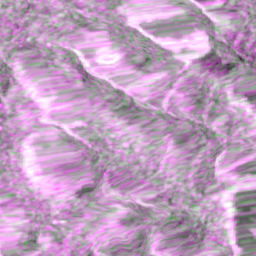
\includegraphics[width=0.2\textwidth, height=0.2\textheight, keepaspectratio]{../latex_source_code/img/cloud_removal/sample_000881_sar_pseudo.png} &
        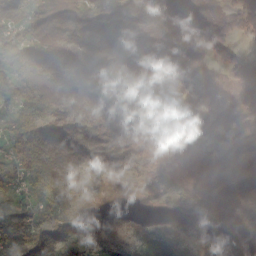
\includegraphics[width=0.2\textwidth, height=0.2\textheight, keepaspectratio]{../latex_source_code/img/cloud_removal/sample_000881_cloudy_rgb.png} &
        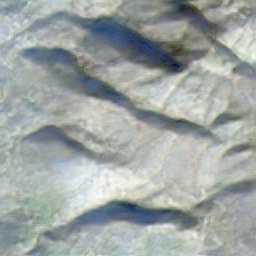
\includegraphics[width=0.2\textwidth, height=0.2\textheight, keepaspectratio]{../latex_source_code/img/cloud_removal/sample_000881_pred_rgb.png} &
        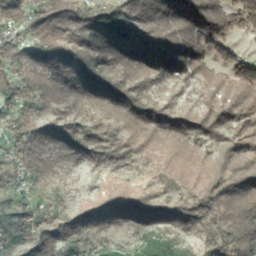
\includegraphics[width=0.2\textwidth, height=0.2\textheight, keepaspectratio]{../latex_source_code/img/cloud_removal/sample_000881_true_rgb.png} \\
        % ------------------- Row 2 -------------------
        \textbf{(b)} &
        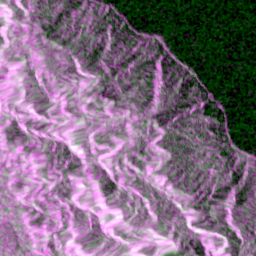
\includegraphics[width=0.2\textwidth, height=0.2\textheight, keepaspectratio]{../latex_source_code/img/cloud_removal/sample_000683_sar_pseudo.png} &
        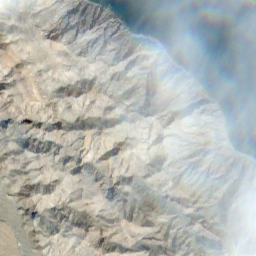
\includegraphics[width=0.2\textwidth, height=0.2\textheight, keepaspectratio]{../latex_source_code/img/cloud_removal/sample_000683_cloudy_rgb.png} &
        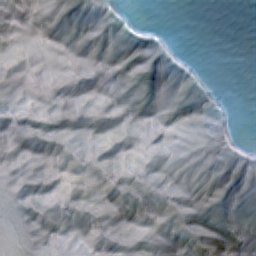
\includegraphics[width=0.2\textwidth, height=0.2\textheight, keepaspectratio]{../latex_source_code/img/cloud_removal/sample_000683_pred_rgb.png} &
        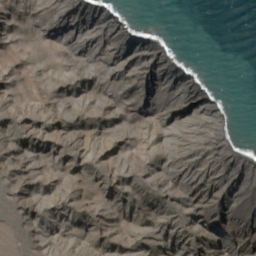
\includegraphics[width=0.2\textwidth, height=0.2\textheight, keepaspectratio]{../latex_source_code/img/cloud_removal/sample_000683_true_rgb.png} \\
        \textbf{(c)} &
        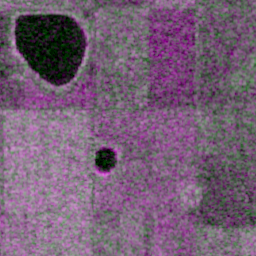
\includegraphics[width=0.2\textwidth, height=0.2\textheight, keepaspectratio]{../latex_source_code/img/cloud_removal/sample_001114_sar_pseudo.png} &
        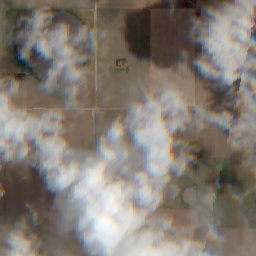
\includegraphics[width=0.2\textwidth, height=0.2\textheight, keepaspectratio]{../latex_source_code/img/cloud_removal/sample_001114_cloudy_rgb.png} &
        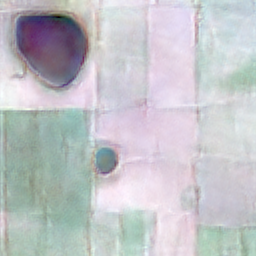
\includegraphics[width=0.2\textwidth, height=0.2\textheight, keepaspectratio]{../latex_source_code/img/cloud_removal/sample_001114_pred_rgb.png} &
        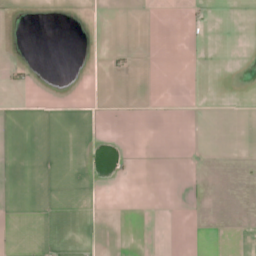
\includegraphics[width=0.2\textwidth, height=0.2\textheight, keepaspectratio]{../latex_source_code/img/cloud_removal/sample_001114_true_rgb.png} \\
        \textbf{(d)} &
        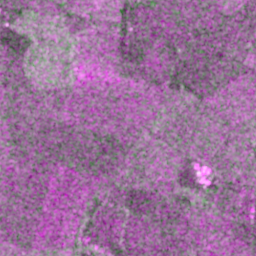
\includegraphics[width=0.2\textwidth, height=0.2\textheight, keepaspectratio]{../latex_source_code/img/cloud_removal/sample_000013_sar_pseudo.png} &
        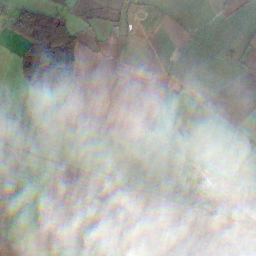
\includegraphics[width=0.2\textwidth, height=0.2\textheight, keepaspectratio]{../latex_source_code/img/cloud_removal/sample_000013_cloudy_rgb.png} &
        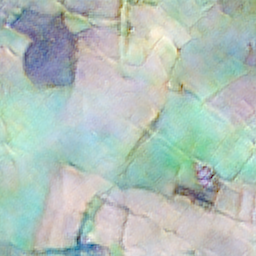
\includegraphics[width=0.2\textwidth, height=0.2\textheight, keepaspectratio]{../latex_source_code/img/cloud_removal/sample_000013_pred_rgb.png} &
        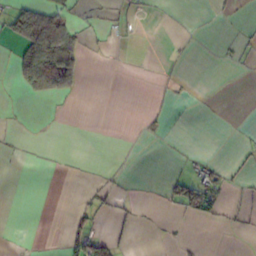
\includegraphics[width=0.2\textwidth, height=0.2\textheight, keepaspectratio]{../latex_source_code/img/cloud_removal/sample_000013_true_rgb.png} \\
        % ------------------- Row 6 -------------------
        \textbf{(e)} &
        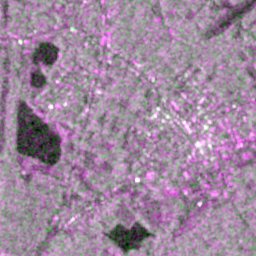
\includegraphics[width=0.2\textwidth, height=0.2\textheight, keepaspectratio]{../latex_source_code/img/cloud_removal/sample_000150_sar_pseudo.png} &
        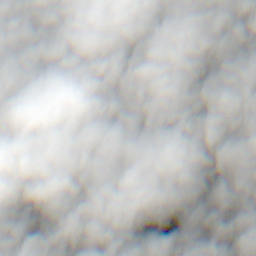
\includegraphics[width=0.2\textwidth, height=0.2\textheight, keepaspectratio]{../latex_source_code/img/cloud_removal/sample_000150_cloudy_rgb.png} &
        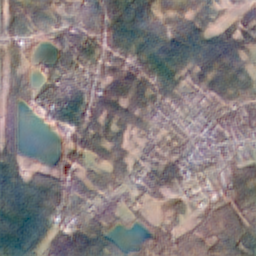
\includegraphics[width=0.2\textwidth, height=0.2\textheight, keepaspectratio]{../latex_source_code/img/cloud_removal/sample_000150_pred_rgb.png} &
        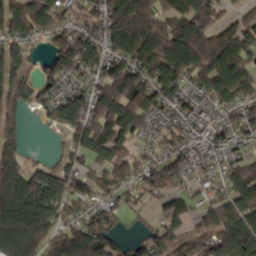
\includegraphics[width=0.2\textwidth, height=0.2\textheight, keepaspectratio]{../latex_source_code/img/cloud_removal/sample_000150_true_rgb.png} \\
    \end{tabular}

    \caption[Qualitative results on cloud removal]{%
    Qualitative results of the model trained on the full winter subset of the SEN12-MS dataset, evaluated on the complementary SEN12-MS-CR dataset for the \textbf{cloud removal} task.  
    Columns: 
    \textbf{(i)}~SAR input (pseudo-RGB; R: VV, G: VH, B: VV/VH), 
    \textbf{(ii)}~reference cloud-contaminated optical image, 
    \textbf{(iii)}~generated cloud-free optical image, and 
    \textbf{(iv)}~reference cloud-free optical image (ground truth).}
    \label{fig:qualitative_results_cloud_removal}
\end{figure}

In summary, both qualitative and quantitative metrics confirm the model’s ability to generate high-quality, cloud-free optical images across all 13 spectral bands. Because the model relies exclusively on SAR input to generate the optical output, the density or presence of clouds in the target area does not influence the reconstruction process, emphasizing the robustness of SAR-to-optical translation in addressing cloud cover.


\subsection{Ablation Studies}
\label{abl:loss}

To assess the individual contributions of the loss functions and spectral bands to the model's reconstruction capability, we conducted two ablation studies. All models were trained using identical hyperparameters and datasets (20\% of the winter subset) to ensure fair comparison.

\subsubsection{Impact of Loss Components}
\label{subsec:ablation_loss}

We evaluated four training configurations to isolate the effects of structural ($\mathcal{L}_{\text{SSIM}}$) and perceptual ($\mathcal{L}_{\text{LPIPS}}$) losses against a baseline adversarial setup:
\begin{enumerate}
    \item $\mathcal{L}_{\text{GAN}} + \mathcal{L}_{\text{L1}}$,
    \item $\mathcal{L}_{\text{GAN}} + \mathcal{L}_{\text{L1}} + \mathcal{L}_{\text{SSIM}}$,
    \item $\mathcal{L}_{\text{GAN}} + \mathcal{L}_{\text{L1}} + \mathcal{L}_{\text{LPIPS}}$, and
    \item the full objective: $\mathcal{L}_{\text{GAN}} + \mathcal{L}_{\text{L1}} + \mathcal{L}_{\text{SSIM}} + \mathcal{L}_{\text{LPIPS}}$.
\end{enumerate}

Table~\ref{tab:ablation_quantitative} summarizes the quantitative results. The baseline configuration ($\mathcal{L}_{\text{GAN}} + \mathcal{L}_{\text{L1}}$) yields the lowest performance across most metrics. This deficiency is also visually apparent, as the generated images lack textural detail (see Fig.~\ref{fig:ablation_samples}b).

Integrating $\mathcal{L}_{\text{SSIM}}$ yields the highest quantitative scores for SSIM and PSNR. However, qualitative inspection reveals that this configuration suffers from perceptual inconsistencies and reduced realism (Fig.~\ref{fig:ablation_samples}c). This aligns with prior findings that SSIM may overemphasize low-level intensity matching at the expense of high-frequency texture fidelity~\cite{nvidia_Understanding_SSIM}. Conversely, incorporating $\mathcal{L}_{\text{LPIPS}}$ significantly improves edge retention and textural realism (Fig.~\ref{fig:ablation_samples}d), reflected in the best LPIPS score of 0.213, though at the cost of slight color deviations compared to the SSIM-based model.

The full combination of losses achieves the optimal trade-off. It maintains competitive pixel-level accuracy (MAE/RMSE) while ensuring structural coherence and perceptual realism, as evidenced in Fig.~\ref{fig:ablation_samples}(e). However, it introduces slight smoothing compared to the LPIPS-only configuration, a tendency likely driven by $\mathcal{L}_{\text{SSIM}}$. This confirms the necessity of a composite loss function that balances the sharpening effect of LPIPS with the structural regularization of SSIM for effective SAR-to-optical translation, consistent with Similar results reported in~\cite{s2o_ViT_cGAN, CR_RS_GAN_s2o}.

\begin{table}[!htbp]
    \centering
    \caption{Quantitative ablation results across loss configurations. Best values are in \textbf{bold}.}
    \label{tab:ablation_quantitative}
    % \resizebox{\columnwidth}{!}{%
        \begin{tabular}{lcccccc}
            \toprule
            \textbf{Configuration} & \textbf{SSIM $\uparrow$} & \textbf{PSNR $\uparrow$} & \textbf{LPIPS $\downarrow$} & \textbf{SAM~(°) $\downarrow$} & \textbf{MAE $\downarrow$} & \textbf{RMSE $\downarrow$} \\
            \midrule
            $\mathcal{L}_{\text{GAN}} + \mathcal{L}_{\text{L1}}$ & 0.820 & 26.38 & 0.287 & 7.88 & 229 & 441 \\
            + $\mathcal{L}_{\text{SSIM}}$ & \textbf{0.862} & \textbf{27.67} & 0.399 & \textbf{6.67} & 198 & \textbf{380} \\
            + $\mathcal{L}_{\text{LPIPS}}$ & 0.842 & 27.58 & \textbf{0.213} & 7.05 & 201 & 385 \\
            Full Combination & 0.859 & 27.65 & 0.224 & 6.71 & \textbf{195} & 382 \\
            \bottomrule
        \end{tabular}%
    % }
\end{table}

\begin{figure}[!htbp]
    \centering
    \setlength{\tabcolsep}{1pt}
    \renewcommand{\arraystretch}{0.5}
    % Grid: 6 columns, responsive width
    \begin{tabular}{cccccc}
        \scriptsize (a) SAR & \scriptsize (b) Base & \scriptsize (c) +SSIM & \scriptsize (d) +LPIPS & \scriptsize (e) Full & \scriptsize (f) GT \\
        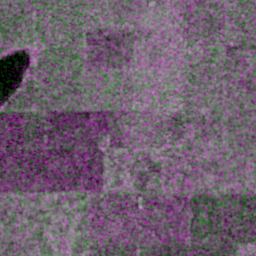
\includegraphics[width=0.16\columnwidth]{../latex_source_code/img/ablation/sample_1/sar.png} &
        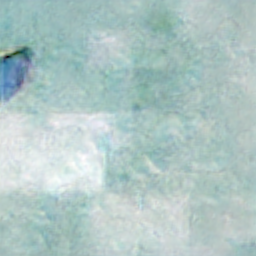
\includegraphics[width=0.16\columnwidth]{../latex_source_code/img/ablation/sample_1/none.png} &
        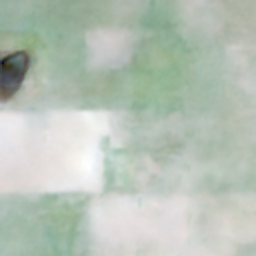
\includegraphics[width=0.16\columnwidth]{../latex_source_code/img/ablation/sample_1/ssim.png} &
        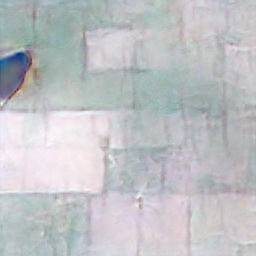
\includegraphics[width=0.16\columnwidth]{../latex_source_code/img/ablation/sample_1/lpips.png} &
        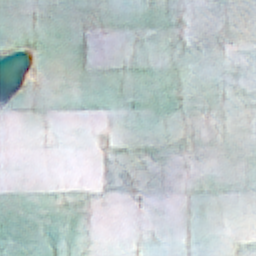
\includegraphics[width=0.16\columnwidth]{../latex_source_code/img/ablation/sample_1/all.png} &
        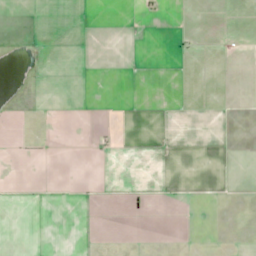
\includegraphics[width=0.16\columnwidth]{../latex_source_code/img/ablation/sample_1/gt.png} \\
        
        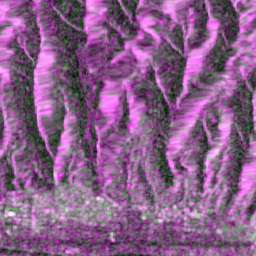
\includegraphics[width=0.16\columnwidth]{../latex_source_code/img/ablation/sample_2/sar.png} &
        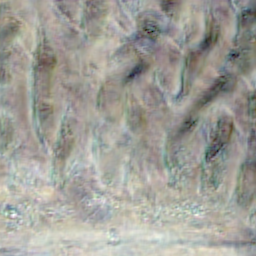
\includegraphics[width=0.16\columnwidth]{../latex_source_code/img/ablation/sample_2/none.png} &
        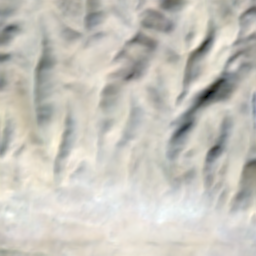
\includegraphics[width=0.16\columnwidth]{../latex_source_code/img/ablation/sample_2/ssim.png} &
        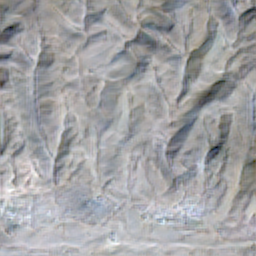
\includegraphics[width=0.16\columnwidth]{../latex_source_code/img/ablation/sample_2/lpips.png} &
        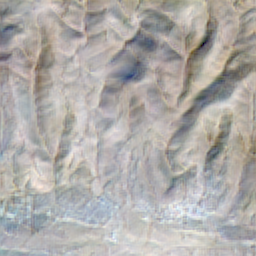
\includegraphics[width=0.16\columnwidth]{../latex_source_code/img/ablation/sample_2/all.png} &
        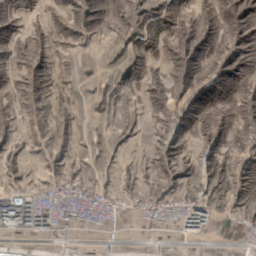
\includegraphics[width=0.16\columnwidth]{../latex_source_code/img/ablation/sample_2/gt.png} \\
        
        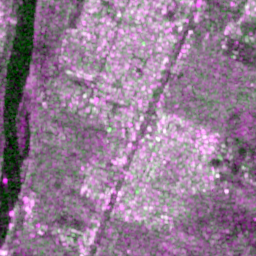
\includegraphics[width=0.16\columnwidth]{../latex_source_code/img/ablation/sample_3/sar.png} &
        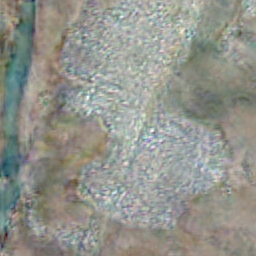
\includegraphics[width=0.16\columnwidth]{../latex_source_code/img/ablation/sample_3/none.png} &
        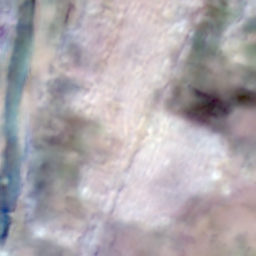
\includegraphics[width=0.16\columnwidth]{../latex_source_code/img/ablation/sample_3/ssim.png} &
        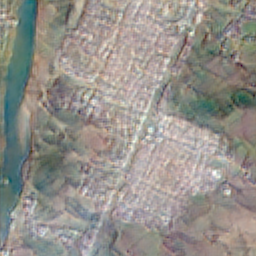
\includegraphics[width=0.16\columnwidth]{../latex_source_code/img/ablation/sample_3/lpips.png} &
        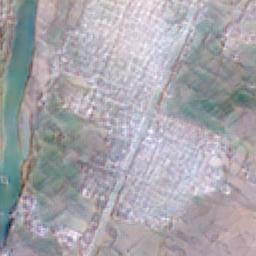
\includegraphics[width=0.16\columnwidth]{../latex_source_code/img/ablation/sample_3/all.png} &
        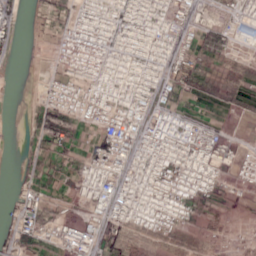
\includegraphics[width=0.16\columnwidth]{../latex_source_code/img/ablation/sample_3/gt.png} \\
    \end{tabular}
    \caption{Visual comparison of loss configurations. (a) Input SAR, (b) Baseline ($\mathcal{L}_{\text{GAN}}{+}\mathcal{L}_{\text{L1}}$), (c) Baseline w/ SSIM, (d) Baseline w/ LPIPS, (e) Proposed full loss, (f) Ground Truth.}
    \label{fig:ablation_samples}
\end{figure}

\subsubsection{Influence of 60m Spectral Bands}
\label{subsec:ablation_60m}
Sentinel-2 includes three 60\,m resolution bands (B1, B9, B10) primarily used for atmospheric correction. We hypothesized that including these lower-resolution bands might introduce noise or training instability due to upsampling artifacts, since they were resampled to 10\,m. To test this, we trained a model strictly excluding these bands.

Contrary to this hypothesis, excluding the 60\,m bands did not improve performance. Instead, radiometric fidelity decreased, with both SSIM and PSNR dropping compared to the full 13-band model (Table~\ref{tab:ablation_excluding_60m}). Interestingly, the Spectral Angle Mapper (SAM) score improved slightly when excluding these bands (6.33° vs. 6.71°). This indicates a trade-off: the model trained on fewer bands learned tighter spectral relationships among the remaining subsets (improving SAM) but lacks the enhanced image quality derived from the atmospheric correction information in the 60\,m bands. It is worth noting, however, that these differences are marginal. Similarly, qualitative inspection in Figure~\ref{fig:ablation_excluding_60m_qualitative} reveals only subtle differences in favour of including the full spectrum.

\begin{table}[!htbp]
    \centering
    \caption{Performance comparison: All 13 bands vs. excluding 60\,m bands (B1, B9, B10).}
    \label{tab:ablation_excluding_60m}
    \begin{tabular}{lccc}
        \toprule
        \textbf{Setting} & \textbf{SSIM $\uparrow$} & \textbf{PSNR (dB) $\uparrow$} & \textbf{SAM~(°) $\downarrow$} \\
        \midrule
        All 13 bands & \textbf{0.859} & \textbf{27.65} & 6.71 \\
        Excluding 60m & 0.826 & 26.47 & \textbf{6.33} \\
        \bottomrule
    \end{tabular}
\end{table}

\begin{figure}[!htbp]
    \centering
    \setlength{\tabcolsep}{2pt}
    \renewcommand{\arraystretch}{0.5}
    \begin{tabular}{cccc}
        \scriptsize (a) SAR & \scriptsize (b) No 60m & \scriptsize (c) Full (13 Bands) & \scriptsize (d) GT \\
        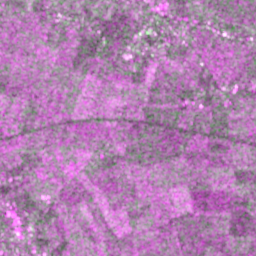
\includegraphics[width=0.23\columnwidth]{../latex_source_code/img/exclusion_60_m/bands10/sample_000034_sar_pseudo.png} &
        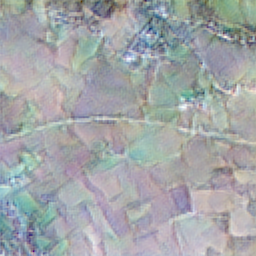
\includegraphics[width=0.23\columnwidth]{../latex_source_code/img/exclusion_60_m/bands10/sample_000034_pred_rgb.png} &
        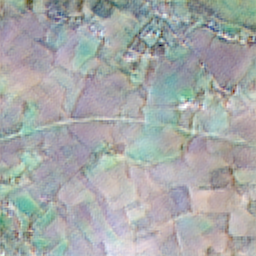
\includegraphics[width=0.23\columnwidth]{../latex_source_code/img/exclusion_60_m/bands13/sample_000034_pred_rgb.png} &
        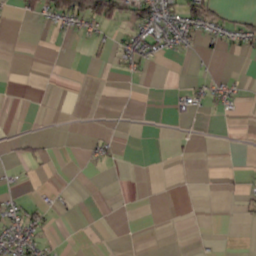
\includegraphics[width=0.23\columnwidth]{../latex_source_code/img/exclusion_60_m/bands10/sample_000034_true_rgb.png} \\
        
        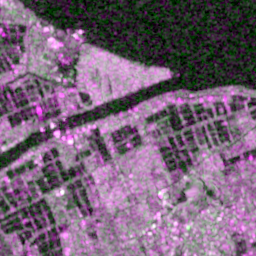
\includegraphics[width=0.23\columnwidth]{../latex_source_code/img/exclusion_60_m/bands10/sample_000050_sar_pseudo.png} &
        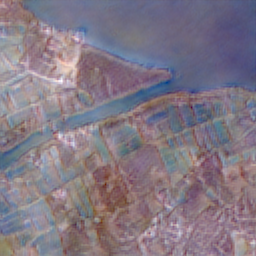
\includegraphics[width=0.23\columnwidth]{../latex_source_code/img/exclusion_60_m/bands10/sample_000050_pred_rgb.png} &
        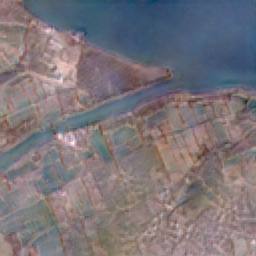
\includegraphics[width=0.23\columnwidth]{../latex_source_code/img/exclusion_60_m/bands13/sample_000050_pred_rgb.png} &
        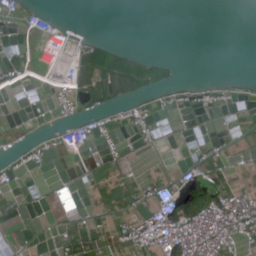
\includegraphics[width=0.23\columnwidth]{../latex_source_code/img/exclusion_60_m/bands10/sample_000050_true_rgb.png} \\
        
         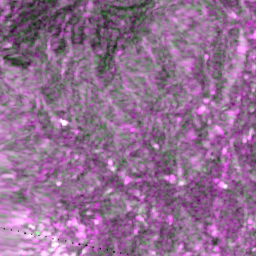
\includegraphics[width=0.23\columnwidth]{../latex_source_code/img/exclusion_60_m/bands10/sample_000010_sar_pseudo.png} &
        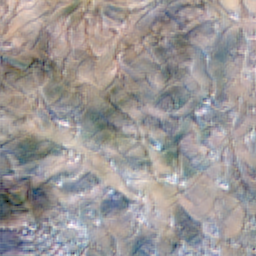
\includegraphics[width=0.23\columnwidth]{../latex_source_code/img/exclusion_60_m/bands10/sample_000010_pred_rgb.png} &
        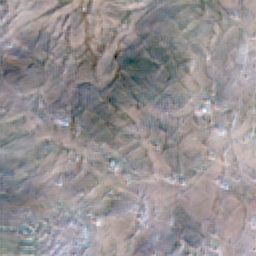
\includegraphics[width=0.23\columnwidth]{../latex_source_code/img/exclusion_60_m/bands13/sample_000010_pred_rgb.png} &
        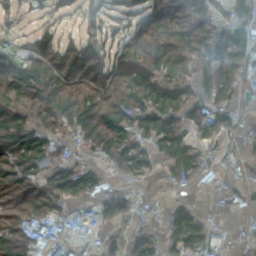
\includegraphics[width=0.23\columnwidth]{../latex_source_code/img/exclusion_60_m/bands10/sample_000010_true_rgb.png} \\
    \end{tabular}
    \caption{Qualitative results comparing models trained with and without the 60\,m bands. (a) SAR input, (b) 10-band model output, (c) 13-band model output, (d) Ground Truth.}
    \label{fig:ablation_excluding_60m_qualitative}
\end{figure}

This trend is further confirmed by the per-band analysis in Table~\ref{tab:ablation_excluding_60m_per_band}. While SSIM remains relatively stable across configurations, PSNR drops for nearly all 10\,m and 20\,m bands when the atmospheric bands are removed, although the absolute differences are small.

\begin{table}[!htbp]
    \centering
    \caption{Per-band performance comparison. \textbf{No 60m}: Model trained without B1, B9, B10. \textbf{13}: Full model.}
    \label{tab:ablation_excluding_60m_per_band}
    \begin{tabular}{lcccc}
    \toprule
    \textbf{Band} & \textbf{SSIM (No 60m)} & \textbf{SSIM (13)} & \textbf{PSNR (No 60m)} & \textbf{PSNR (13)} \\
    \midrule
    B1   & ---    & 0.9634 & ---    & 29.749 \\
    B2 & \textbf{0.9431} & 0.9430 & \textbf{34.15} & 34.06 \\
    B3 & \textbf{0.9064} & 0.9060 & 31.69 & \textbf{31.72} \\
    B4 & \textbf{0.8348} & 0.8340 & 28.04 & \textbf{28.15} \\
    B5 & 0.8707 & \textbf{0.8729} & 28.10 & \textbf{28.26} \\
    B6 & 0.8199 & \textbf{0.8231} & 26.74 & \textbf{26.93} \\
    B7 & 0.7890 & \textbf{0.7925} & 25.69 & \textbf{25.88} \\
    B8 & 0.7375 & \textbf{0.7416} & 25.53 & \textbf{25.74} \\
    B8A & 0.7687 & \textbf{0.7722} & 25.10 & \textbf{25.31} \\
    B9   & ---    & 0.8666 & ---    & 24.617 \\
    B10  & ---    & 0.8826 & ---    & 24.571 \\
    B11 & 0.7774 & \textbf{0.7809} & 23.40 & \textbf{23.73} \\
    B12 & 0.8034 & \textbf{0.8073} & 24.96 & \textbf{25.26} \\
    \bottomrule
    \end{tabular}
\end{table}

